
We will now focus on measurable functions $M\to \overline{\R}$ and define their integral on a subset of $M$ with respect to some measure on $M$, which is called the Lebesgue integral. Note that, even if $M\subseteq\R^d$, the Lebesgue integral of a function need not be with respect to the Lebesgue measure. 

The key application of this material is the definition of the Banach spaces of (classes of) Lebesgue integrable functions $L^p$. The case $p=2$ is especially important since $L^2$ is, in fact, a Hilbert space. It appears a lot in quantum mechanics where it is loosely referred to as the space of square-integrable functions.

\section{Characteristic and simple functions}

\begin{definition}
Let $M$ be a set and let $A\in\mathscr{P}(M)$. The
\emph{characteristic function}\index{characteristic function} of $A$,
denoted $\chi_A\cl M\to \R$, is defined by
\begin{equation*}
  \chi_A(m)
  =
  \begin{cases}
    1 & \text{if } m\in A \\
    0 & \text{if } m\notin A.
  \end{cases}
\end{equation*}
\end{definition}

\begin{example}
Below is the graph of $\chi_{(1,2]}\cl \R \to \R$.
\begin{center}
\begin{tikzpicture}[scale=1.2]
\draw[->] (0,-0.5)--(0,1.75);
\draw[->] (-0.5,0)--(3.5,0);
\foreach \i in {1,2,3}{
\draw (\i,0.08)--(\i,-0.08) node[below=2pt] {$\i$};
}
\draw (0.08,1) -- (-0.08,1) node[left] {$1$};
\draw (0,0) node[below left] {$0$};
\draw (1,1)--(2,1) node[right=3pt] {$\chi_{(1,2]}$};
\draw[dotted] (0,1)--(1,1)--(1,0);
\draw[dotted] (2,1)--(2,0);
\draw[fill=white] (1,1) circle [radius=0.08];
\draw[fill] (2,1) circle [radius=0.08];
\end{tikzpicture}
\end{center}
\end{example}

The following properties of characteristic functions are immediate.
\begin{proposition}
\label{prp:characteristic}
Let $M$ be a set and let $A,B\in\mathscr{P}(M)$. Then
\begin{enumerate}[label=(\roman*)]
\item $\chi_{\varnothing}=0$
\item $\chi_{A\cup B} = \chi_A+\chi_B-\chi_{A\cap B}$
\item $\chi_{A\cap B} = \chi_A\chi_B$
\item $\chi_{M\setminus A} + \chi_A = 1$
\end{enumerate}
where the addition and multiplication are pointwise and the $0$ and
$1$ in parts (i) and (iv) are the constant functions $M\to \R$ mapping
every $m\in M$ to $0\in\R$ and $1\in\R$, respectively.
\end{proposition}

\begin{definition}
Let $M$ be a set. A function $s\cl M \to \R$ is
\emph{simple}\index{simple function} if $s(M)$ is a finite set.
%Let $(M,\Sigma)$ be a measurable space. A measurable function $s\cl M
%\to \R$ is said to be \emph{simple}\index{simple function} if $s(M) =
%\{r_1,\ldots,r_n\}$ for some $n\in \N$.
\end{definition}

Simple functions form a vector space. Since the caracteristic
functions \(\chi_A\) are always simple, any finite linear combination
\begin{equation}
  \label{eq:sumchar}
  s = \sum_{i=1}^nr_i\chi_{A_i}
\end{equation}
is also a simple function.
Conversely, if \(s\) is a simple function with range
\(s(M)=\{r_1,\dots,r_n\}\) and \(A_i=s^{-1}(r_i)\), then it admits an
expression as in \eqref{eq:sumchar},
where the sets \(A_i\) satisfy the additional condition
\(A_i\cap A_j=\emptyset\) whenever \(i\neq j\).
An expression satisfying this condition is said to be a \emph{standard
form} of \(s\).

Moreover, suppose that \((M,\Sigma)\) is a measurable space.
If \(A_1,\dots,A_n\) are measurable sets, then the function
\eqref{eq:sumchar} is measurable. Conversely, if \(s\) is measurable
with range \(s(M)=\{r_1,\dots,r_n\}\), then each \(A_i=s^{-1}(r_i)\)
is measurable. We also have the following proposition.

\begin{proposition}
Let $(M,\Sigma)$ be a measurable space and $s=\sum_{i=1}^n r_i
\chi_{A_i}$ a simple function in standard form.
Then $s$ is measurable if, and only if, we have $A_i\in \Sigma$ for
all $1\leq i\leq n$.
\end{proposition}

\begin{example}
Consider the simple function $s\cl \R \to \R$ given by
$s:=\chi_{[1,3]}+2\chi_{[2,5]}$.
\begin{center}
\begin{tikzpicture}[scale=1.2]
\draw[->] (0,-0.5)--(0,3.75);
\draw[->] (-0.5,0)--(5.75,0);
\foreach \i in {1,2,3,4,5}{
\draw (\i,0.08)--(\i,-0.08) node[below=2pt] {$\i$};
}
\foreach \i in {1,2,3} {
\draw (0.08,\i) -- (-0.08,\i) node[left] {$\i$};
}
\draw (0,0) node[below left] {$0$};
\draw (1,1)--(2,1);
\draw (2,3)--(3,3);
\draw (3,2)--(5,2);
\draw[dotted] (0,1)--(1,1)--(1,0);
\draw[dotted] (0,3)--(2,3)--(2,0);
\draw[dotted] (0,2)--(3,2);
\draw[dotted] (3,3)--(3,0);
\draw[dotted] (5,2)--(5,0);
\draw[fill] (1,1) circle [radius=0.08];
\draw[fill=white] (2,1) circle [radius=0.08];
\draw[fill] (3,3) circle [radius=0.08];
\draw[fill] (2,3) circle [radius=0.08];
\draw[fill] (5,2) circle [radius=0.08];
\draw[fill=white] (3,2) circle [radius=0.08];
\end{tikzpicture}
\end{center}
By observing the graph, we see that a standard form of $s$ is
\begin{equation*}
s = \chi_{[1,2)} + 3 \chi_{[2,3]} + 2 \chi_{(3,5]}.
\end{equation*}
\end{example}

\section{\texorpdfstring{
  Integration of non-negative \\ measurable simple functions}
  {Integration of non-negative measurable simple functions}}

We begin with the definition of the integral of a non-negative,
measurable, simple function.

\begin{definition}
  Let $(M,\Sigma,\mu)$ be a measure space and let $s\cl M \to \R$ be a
  nowhere negative, measurable, simple function.
  Let $s=\sum_{i=1}^n r_i \chi_{A_i}$ be a standard form of \(s\).
  Then, we define
  \begin{equation}
    \label{eq:intsimp}
    \int_M \! s \, \d \mu := \sum_{i=1}^nr_i\mu(A_i).
  \end{equation}
\end{definition}

Note that the non-negativity condition is essential since $\mu$ takes
values in $[0,\infty]$, hence we could have $\mu(A_i)=\infty$ for more
that one $A_i$, and if the corresponding coefficients $r_i$ have
opposite signs, then we would have $\int_Ms\,\d\mu=\infty-\infty$,
which is not defined. For the same reason, we are considering $s\cl
M\to [0,\infty)$ rather than $s\cl M\to [0,\infty]$.

\begin{remark}
  The definition of \(\int_M s\d\mu\) is independent of the choice of
  standard form of \(s\). Moreover, the following lemma implies that
  the expression \(s=\sum_{i=1}^{n}r_i\chi_{A_i}\) doesn't even need
  to be a standard form of \(s\), and the expression
  \eqref{eq:intsimp} also calculates the integral of \(s\).
\end{remark}

\begin{lemma}
  \label{lem:simplelinear}
  Let $(M,\Sigma,\mu)$ be a measure space. Let $s$ and $t$ be
  non-negative, measurable, simple functions $M\to \R$ and let $c\in
  [0,\infty)$. Then
  \begin{equation}
  \int_M(cs+t)\d\mu = c\int_Ms\d\mu+\int_Mt\d\mu.
  \end{equation}
  Moreover, if \(s\leq t\), then
  \begin{equation}
    \int_Ms\d\mu \leq \int_Mt\d\mu
  .\end{equation}
\end{lemma}

\begin{example}
  Consider the measure space $(\N,\mathscr{P}(\N),\mu)$, where $\mu$
  is the counting measure, let $f\cl \N \to \R$ be non-negative and
  suppose that there exists $N\in\N$ such that $f(n)=0$ for all $n>N$.
  Then, we can write $f$ as
  \begin{equation*}
  f=\sum_{n=0}^Nf(n)\chi_{\{n\}}.
  \end{equation*}
  That is, $f$ is a non-negative, measurable, simple function and therefore
  \begin{equation*}
  \int_{\N}\! f \,\d \mu := \sum_{n=0}^Nf(n)\mu(\{n\}) = \sum_{n=0}^Nf(n).
  \end{equation*}
  Hence, the ``integral'' of $f$ over $\N$ with respect to the counting measure is just the sum.
\end{example}

\begin{lemma}
Let $(M,\Sigma, \mu)$ be a measure space and let $s = \sum_{i=1}^n{r_i\chi_{A_i}}$ be a non-negative, measurable, simple function $M\to\R$. Define the map
\begin{IEEEeqnarray*}{rrCl}
\nu_s \cl & \Sigma & \to & [0,\infty]\\
& A & \mapsto &  \int_M \! s\chi_A \, \d \mu,
\end{IEEEeqnarray*}
where $s\chi_A$ is the pointwise product of $s$ and $\chi_A$. Then, $\nu_s$ is a measure on $(M,\Sigma)$.
\end{lemma}

\begin{proof}
First, note that we have
\begin{equation*}
\int_M \! s\chi_A \, \d \mu
= \int_M \sum_{\,i=1}^nr_i\chi_{A_i}\chi_{A} \d \mu
= \int_M \sum_{\,i=1}^nr_i\chi_{A_i\cap A} \d \mu
=\sum_{i=1}^nr_i\mu({A_i\cap A)}.
\end{equation*}
We now check that $\nu$ satisfies the defining properties of a measure.
\begin{enumerate}[label=(\roman*)]
\item $\displaystyle\nu_s(\varnothing):= \int_M \! s\chi_{\varnothing} \, \d \mu = \sum_{i=1}^n{r_i\mu({A_i\cap \varnothing})} = \sum_{i=1}^n{r_i\mu(\varnothing)} = 0$
\item Let $\{B_j\}_{j\in\N}$ be a pairwise disjoint sequence in $\Sigma$. Then
\begin{IEEEeqnarray*}{rCl}
\nu_s \biggl( \bigcup_{\,j=0}^{\infty}B_j \biggr) &=& \int_M \! s\chi_{ \left( \bigcup_{j=0}^{\infty}B_j \right)} \, \d \mu \\
& = & \sum_{i=1}^n r_i  \mu \biggl( \bigcup_{\,j=0}^{\infty}(A_i \cap B_j )\biggr)\\
&=& \sum_{j=0}^{\infty}\sum_{i=1}^n r_i \mu (A_i \cap B_j )\\
&=& \sum_{j=0}^{\infty}\int_M \! s\chi_{B_j} \, \d \mu \\
&=& \sum_{j=0}^{\infty}\nu_s(B_j) .
\end{IEEEeqnarray*}
\end{enumerate}
Thus, $\nu_s$ is a measure on $(M,\Sigma)$. \qedhere
\end{proof}

\section{Integration of non-negative measurable functions}

As we are interested in measurable functions $M\to\overline{\R}$, we need to define a $\sigma$-algebra on $\overline{\R}$. We cannot use the Borel $\sigma$-algebra since we haven't even defined a topology on $\overline{\R}$. In fact, we can easily get a $\sigma$-algebra on $\overline{\R}$ as follows.

\begin{proposition}
The set $\overline{\Sigma}:=\{A\in \mathscr{P}(\overline{\R})\mid A\cap \R \in \sigma(\mathcal{O}_{\R})\}$ is a $\sigma$-algebra on $\overline{\R}$.
\end{proposition}
In other words, we can simply ignore the infinities in a subset of
$\overline{\R}$ and consider it to be measurable if
$A\setminus\{-\infty,+\infty\}$ is in the Borel $\sigma$-algebra of
$\R$. We will always consider $\overline{\R}$ to be equipped with this
$\sigma$-algebra.

\begin{lemma}
\label{lem:measurable}
Let $(M,\Sigma)$ be a measurable space and let $f,g\cl M\to
\overline{\R}$ be measurable. Then, the following functions are
measurable.
\begin{enumerate}[label=(\roman*)]
\item $cf+g$, for any $c\in \R$
\item $|f|$ and $f^2$
\item $fg$ (pointwise product) if $f$ and $g$ are nowhere infinite
\item $\max(f,g)$ (defined pointwise).
\end{enumerate}
\end{lemma}

\begin{definition}
  Let $(M,\Sigma,\mu)$ be a measure space and let $f\cl
  M\to\overline{\R}$ be a non-negative, measurable function.
  Then, we define
  \begin{equation*}
    \int_Mf\d \mu
    :=
    \sup\left\{
      \int_M s \d \mu : s \text{ is simple, measurable and } 0\leq s\leq f
    \right\}
  \end{equation*}
\end{definition}

\begin{remark}
It is often very convenient to introduce the notation
\begin{equation*}
\int_M\!f(x)\,\mu(\d x) \equiv \int_M\! f\, \d \mu,
\end{equation*}
where $x$ is a dummy variable and could be replaced by any other
symbol. The reason why this is a convenient notation is that, while
some functions have standard symbols but cannot be easily represented
by an algebraic expression (e.g. characteristic functions), others are
easily expressed in terms of an algebraic formula but do not have a
standard name. For instance, it is much easier to just write
\begin{equation*}
\int_{\R}  x^2\,\mu(\d x)
\end{equation*}
than having to first denote the function $\R\to\R$, $x\mapsto x^2$ by
a generic $f$ or, say, the more specific $\mathrm{sq}_{\R}$, and then
write
\begin{equation*}
\int_\R\mathrm{sq}_{\R}\, \d \mu.
\end{equation*}
In computer programming, this is akin to defining \emph{anonymous functions}.
\end{remark}

\begin{definition}
  Let $(M,\Sigma,\mu)$ be a measure space and let $f\cl
  M\to\overline{\R}$ be a non-negative, measurable function. For any
  $A\in \Sigma$ (that is, any measurable subset of $M$), we define
  \begin{equation*}
  \int_A\! f\, \d \mu := \int_M\! f\chi_A\, \d \mu.
  \end{equation*}
\end{definition}
Note that the product $f\chi_A$ is measurable by part (iii) of
\Cref{lem:measurable}.

\begin{lemma}
  \label{lem:intineq}
  Let $(M,\Sigma,\mu)$ be a measure space, let $f,g\cl
  M\to\overline{\R}$ be non-negative, measurable functions and $A,B\in
  \Sigma$ measurable sets. Then
  \begin{enumerate}[label=(\roman*)]
    \item
      If \(f\leq g\), then
      $\displaystyle \int_M\! f\, \d \mu \leq \int_M\! g\, \d \mu$
    \item
      If \(A\subseteq B\), then
      $\displaystyle \int_A\! f\, \d \mu \leq \int_B\! f\, \d \mu$.
  \end{enumerate}
\end{lemma}

\begin{proof}
\begin{enumerate}[label=(\roman*)]
\item Denote by $S_f$ and $S_g$ the sets of non-negative, measurable, simple functions that are less than or equal to $f$ and $g$, respectively. As $f\leq g$, we have $S_f\subseteq S_g$ and hence
\begin{equation*}
\int_M\! f\, \d \mu :=  \sup_{s\in S_f}\, \int_M\! s\, \d \mu \leq \sup_{s\in S_g}\, \int_M\! s\, \d \mu =: \int_M\! g\, \d \mu.
\end{equation*}
\item Since $A\subseteq B$, for any $m\in M$ we have
\begin{equation*}
f(m)\chi_A(m) \leq f(m)\chi_B(m).
\end{equation*}
In fact, we have equality whenever $m\in A$ or $m\in M\setminus B$, while for $m\in B\setminus A$ the left hand side is zero and the right-hand side is non-negative. Hence, $f\chi_A\leq f\chi_B$ and thus, by part (i), we have
\begin{equation*}
\int_A\! f\, \d \mu := \int_M\! f\chi_A\, \d \mu \leq\int_M\! f\chi_B\, \d \mu =: \int_B\! f\, \d \mu \qedhere
\end{equation*}
\end{enumerate}
\end{proof}

\begin{proposition}[Markov inequality]
Let $(M,\Sigma,\mu)$ be a measure space and let $f\cl M\to\overline{\R}$ be a non-negative, measurable function. For any $z\in [0,\infty]$, we have
\begin{equation*}
\int_M\! f\, \d \mu \geq z\, \mu(\preim_f([z,\infty])).
\end{equation*}
\end{proposition}

Equality is achieved whenever $z$ is an upper bound for $f$.

\begin{center}
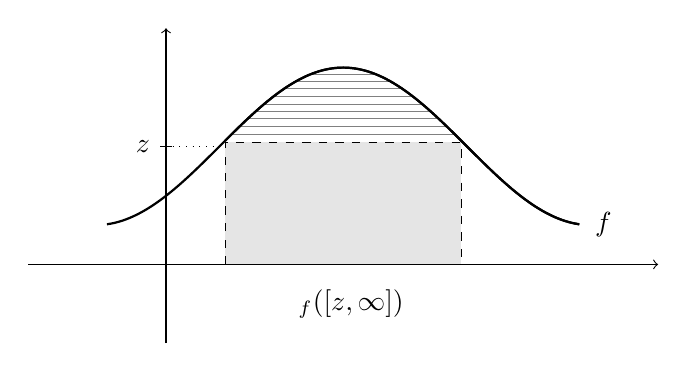
\begin{tikzpicture}
\foreach \i in {0.25,0.6,0.95,1.3,1.65,2.05,2.5,3,3.55} {
\draw[gray] (-0.5+0.3*\i,{1.5+cos deg (-0.5+0.3*\i-1)}) -- (2.5-0.3*\i,{1.5+cos deg (2.5-0.3*\i-1)}) ;
}
\fill[black!10!white] (-0.5,0) rectangle (2.5,1.55);
\draw[dashed,thin] (-0.5,0)--(-0.5,1.55)--(2.5,1.55)--(2.5,0);
\draw (-1.17,1.5)--(-1.33,1.5) node[left] {$z$};
\draw (1.1,-0.5) node {$\preim_f([z,\infty])$};
\draw[dotted] (-1.25,1.5)--(-0.5,1.5);
\draw [thick,smooth,samples=100,variable=\x,domain=-2:4] plot(\x,{1.5+cos deg (\x-1)}) node[right=2pt] {$f$};
\draw [thick,smooth,samples=100,variable=\x,domain=-0.5:4] plot(\x,{1.5+cos deg (\x-1)});
\draw[->,thin] (-3,0)--(5,0);
\draw[->,thin] (-1.25,-1)--(-1.25,3);
\end{tikzpicture}
\end{center}

The following is the pivotal theorem of Lebesgue integration.

\begin{theorem}[Monotone convergence theorem]
Let $(M,\Sigma,\mu)$ be a measure space and let $\{f_n\}_{n\in\N}$ be a sequence of non-negative, measurable functions $M\to\overline{\R}$ such that $f_{n+1}\geq f_n$ for all $n\in \N$. If there exists a function $f\cl M\to \overline{\R}$ such that
\begin{equation*}
\forall \, m \in M : \ \lim_{n\to\infty}f_n(m) = f(m)
\end{equation*}
(i.e. $f$ is the pointwise limit of  $\{f_n\}_{n\in\N}$), then $f$ is measurable and
\begin{equation*}
\lim_{n\to\infty}\int_M\! f_n \, \d \mu = \int_M\! f \, \d \mu.
\end{equation*}
\end{theorem}

\begin{remark}
Observe that this result is in stark contrast with what one may be used from Riemann integration, where pointwise converge of a sequence of integrable functions $\{f_n\}_{n\in\N}$ is \emph{not} a sufficient condition for the integral of the limit $f$ to be equal to the limit of the integrals of $f_n$ or, in fact, even for $f$ to be integrable. For these, we need stronger conditions on the sequence $\{f_n\}_{n\in\N}$, such as uniform converge.
\end{remark}

The definition of the integral as a supremum is clear and geometrically reasonable. However, it is in general very difficult to evaluate
the integral of any particular function using it. The monotone convergence theorem provides a much simpler way to evaluate the integral. One can show that, for any non-negative, measurable function $f$, there exists an increasing sequence $\{s_n\}_{n\in\N}$ of non-negative, measurable, simple functions (which can be explicitly constructed from $f$) whose pointwise limit is $f$, and hence we have
\begin{equation*}
\int_M\! f \, \d \mu = \lim_{n\to\infty}\int_M\! s_n \, \d \mu,
\end{equation*}
where the right-hand side can usually be evaluated fairly easily.

\begin{example}
Consider the measure space $(\N,\mathscr{P}(\N),\mu)$, where $\mu$ is the counting measure, and let $f\cl \N \to \overline{\R}$ be non-negative. Note that the choice of $\sigma$-algebra $\mathscr{P}(\N)$ on $\N$ makes every function on $\N$ (to any measurable space) measurable. Define, for every $n\in \N$,  
\begin{equation*}
s_n=\sum_{i=0}^nf(i)\chi_{\{i\}}.
\end{equation*}
Then, $\{s_n\}_{n\in\N}$ is an increasing sequence of non-negative, measurable, simple functions whose pointwise limit is $f$ and therefore, by the monotone convergence theorem,
\begin{equation*}
\int_{\N}\! f \,\d \mu =\lim_{n\to\infty}\int_{\N}\! s_n \, \d \mu = \lim_{n\to\infty}\sum_{i=0}^nf(i)\mu(\{i\}) = \sum_{i=0}^{\infty}f(i).
\end{equation*}
If you every wondered why series seem to share so many properties with integrals, the reason is that series are just integrals with respect to a discrete measure.
\end{example}

The monotone convergence theorem can be used to extend some of properties of integrals of non-negative, measurable simple functions to non-negative, measurable functions which are not-necessarily simple.

\begin{lemma}
Let $(M,\Sigma,\mu)$ be a measure space, let $f,g\cl M\to \overline{\R}$ be non-negative, measurable functions and let $c\in [0,\infty)$. Then
\begin{enumerate}[label=(\roman*)]
\item $\displaystyle \int_{M}\! (cf+g) \,\d \mu = c\int_{M}\! f \,\d \mu +\int_{M}\! g \,\d \mu $
\item the map $\nu_f\cl \Sigma\to [0,\infty]$ defined by $\displaystyle \nu_f(A):=\int_A\, f\, \d \mu$ is a measure on $(M,\Sigma)$
\item for any $A\in\Sigma$, we have $\displaystyle \int_{M}\!f \,\d \mu =  \int_{A}\!f \,\d \mu+ \int_{M\setminus A}\!f \,\d \mu$.
\end{enumerate}
\end{lemma}

\begin{proof}
\begin{enumerate}[label=(\roman*)]
\item Let $\{s_n\}_{n\in\N}$ and $\{t_n\}_{n\in\N}$ be increasing sequences of non-negative, measurable, simple functions whose pointwise limits are $f$ and $g$, respectively. Then, it is easy to see that $\{cs_n+t_n\}_{n\in\N}$ is an increasing sequence of non-negative, measurable, simple functions whose pointwise limit is $cf+g$. Hence, by \Cref{lem:simplelinear} and the monotone converge theorem
\begin{IEEEeqnarray*}{rCl}
\int_M\! (cf+g) \,\d \mu & = &  \lim_{n\to\infty}\int_M\! (cs_n+t_n) \, \d \mu\\
& = &  \lim_{n\to\infty}\biggl(c\int_M\! s_n \, \d \mu+\int_M\! t_n \, \d \mu\biggr)\\
& = &  c\lim_{n\to\infty}\int_M\! s_n \, \d \mu+\lim_{n\to\infty}\int_M\! t_n \, \d \mu\\
& = &  c\int_{M}\! f \,\d \mu +\int_{M}\! g \,\d \mu.
\end{IEEEeqnarray*}
\item To check that $\nu_f$ is a measure on $(M,\Sigma)$, first note that we have
\begin{equation*}
\nu_f(\varnothing) = \int_{\varnothing}\! f\, \d \mu :=\int_{M}\! f\chi_{\varnothing}\, \d \mu = 0.
\end{equation*}
Let $\{A_i\}_{i\in\N}$ be a pairwise disjoint sequence in $\Sigma$. Define, for any $n\in \N$,
\begin{equation*}
f_n:=f\chi_{\left(\bigcup_{i=0}^nA_i\right)}.
\end{equation*}
Since, for all $n\in \N$, we have $\bigcup_{i=0}^{n}A_i\subseteq\bigcup_{i=0}^{n+1}A_i$ and $f$ is non-negative, $\{f_n\}_{n\in\N}$ is an increasing sequence of non-negative, measurable, simple functions whose pointwise limits is $f\chi_{\left(\bigcup_{i=0}^{\infty}A_i\right)}$. Hence, by recalling \Cref{prp:characteristic}, we have
\begin{IEEEeqnarray*}{rCl}
\nu_f\biggl(\bigcup_{\,i=0}^{\infty}A_i\biggr) & := & \int_{\,\bigcup_{i=0}^{\infty}A_i}\! f \, \d \mu\\
& = & \int_{M} \!f\chi_{\left(\bigcup_{i=0}^{\infty}A_i\right)} \, \d \mu\\
& = & \lim_{n\to\infty}\int_{M} \!f\chi_{\left(\bigcup_{i=0}^{n}A_i\right)} \, \d \mu\\
& = & \lim_{n\to\infty}\int_{M} \biggl(f\sum_{i=0}^{n}\chi_{A_i}\biggr) \, \d \mu\\
& = & \lim_{n\to\infty}\biggl(\sum_{\,i=0}^{n}\int_{M}\! f\chi_{A_i}\, \d \mu\biggr) \\
& = & \sum_{i=0}^{\infty}\nu_f(A_i) .
\end{IEEEeqnarray*}
\item Note that $A\cap (M\setminus A)=\varnothing$. Hence, by using the fact that $\nu_f$ from part (ii) is a measure on $(M,\Sigma)$, we have
\begin{equation*}
\int_M\! f \, \d \mu  =  \nu_f(M) =  \nu_f(A)+\nu_f(M\setminus A) =  \int_A\! f\, \d \mu + \int_{M\setminus A}\! f\, \d \mu. \qedhere
\end{equation*}
\end{enumerate}
\end{proof}

Part (i) of the previous lemma and the monotone convergence theorem also imply that, for any sequence $\{f_n\}_{n\in\N}$ of non-negative, measurable functions, we have
\begin{equation*}
\int_M \biggl(\sum_{\,n=0}^{\infty}f_n \biggr) \d \mu = 
\sum_{n=0}^{\infty} \int_M \! f_n \, \d \mu.
\end{equation*}
Again, note that this result does \emph{not} hold for the Riemann integral unless stronger conditions are places on the sequence $\{f_n\}_{n\in\N}$.

Finally, we have a simple but crucial result for Lebesgue integration.

\begin{theorem}
\label{thm:aezero}
Let $(M,\Sigma,\mu)$ be a measure space and let $f\cl M\to\overline{\R}$ be a non-negative, measurable function. Then
\begin{equation*}
\int_M\! f\, \d \mu = 0 \quad \Leftrightarrow \quad f=_{\mathrm{a.e.}} 0.
\end{equation*}
\end{theorem}

\begin{proof}
\begin{itemize}
\item[$(\Rightarrow)$] Suppose that $\int_Mf\,\d\mu=0$. Define $A_n:=\{m\in M \mid f(m)>\tfrac{1}{n+1}\}$ and let
\begin{equation*}
s_n := \tfrac{1}{n+1}\chi_{A_n} .
\end{equation*}
By definition of $A_n$, we clearly have $s_n\leq f$ for all $n\in\N$. Hence,
\begin{equation*}
0\leq \int_M\!s_n\,\d\mu\leq\int_M\!f\,\d\mu=0
\end{equation*}
and thus, $\int_Ms_n\,\d\mu=0$ for all $n\in\N$. Since by definition
\begin{equation*}
\int_M\!s_n\,\d\mu = \tfrac{1}{n+1}\mu(A_n),
\end{equation*}
we must also have $\mu(A_n)=0$ for all $n\in\N$. Let $A:=\{m\in M \mid f(m)\neq 0\}$. Then, as $f$ is non-negative, we have
\begin{equation*}
A = \bigcup_{n=0}^{\infty}A_n=\bigcup_{n=0}^{\infty}\{m\in M \mid f(m)>\tfrac{1}{n+1}\}
\end{equation*}
and, since $A_n\subseteq A_{n+1}$ for all $n\in\N$, we have
\begin{equation*}
\mu(A)=\mu\biggl(\bigcup_{\,n=0}^{\infty}A_n\biggr)=\lim_{n\to\infty}\mu(A_n) = 0.
\end{equation*}
Thus, $f$ is zero except on the null set $A$. That is, $f=_{\mathrm{a.e.}}0$. 

\item[$(\Leftarrow)$] Suppose that $f=_{\mathrm{a.e.}}0$. Let $S$ be the set of non-negative, measurable, simple functions $s$ such that $s\leq f$. As $f=_{\mathrm{a.e.}}0$, we have $s=_{\mathrm{a.e.}}0$ for all $s\in S$. Thus, if
\begin{equation*}
s=\sum_{i=1}^nr_i\chi_{A_i},
\end{equation*}
we must have either $r_i=0$ or $\mu(A_i)=0$ for all $1\leq i\leq n$. Hence, for all $s\in S$,
\begin{equation*}
\int_M\! s \, \d \mu := \sum_{i=1}^nr_i\mu(A_i) =0.
\end{equation*}
Therefore, we have
\begin{equation*}
\int_M\! f \, \d \mu := \sup_{s\in S}\int_M\! s \, \d \mu  = 0.\qedhere
\end{equation*}
\end{itemize}
\end{proof}

This means that, for the purposes of Lebesgue integration, null sets can be neglected as they do not change the value of an integral. The following are some examples of this.

\begin{corollary}
Let $(M,\Sigma,\mu)$ be a measure space, let $A\in\Sigma$ and let $f,g\cl M\to\overline{\R}$ be non-negative, measurable functions. 
\begin{enumerate}[label=(\roman*)]
\item If $\mu(A)=0$, then $\displaystyle\int_A\! f \, \d \mu = 0$
\item If $f=_{\mathrm{a.e.}}g$, then $\displaystyle\int_M\! f \, \d \mu = \int_M\! g \, \d \mu$
\item If $f\leq_{\mathrm{a.e.}}g$, then $\displaystyle\int_M\! f \, \d \mu \leq \int_M\! g \, \d \mu$.
\end{enumerate}
\end{corollary}

\begin{proof}
\begin{enumerate}[label=(\roman*)]
\item Clearly, $f\chi_A =_{\mathrm{a.e.}}0$ and hence
\begin{equation*}
\int_A\! f \, \d \mu =\int_M\! f\chi_A  \, \d \mu = 0.
\end{equation*}
\item As $f=_{\mathrm{a.e.}}g$, we have $f-g=_{\mathrm{a.e.}}0$ and thus
\begin{equation*}
0 = \int_M\! (f-g) \, \d \mu =\int_M\! f \, \d \mu-\int_M\! g \, \d \mu.
\end{equation*}
\item Let $B:=\{m\in M\mid f(m)>g(m)\}$. As $f\leq_{\mathrm{a.e.}}g$, we have $\mu(B)=0$ and $f\leq g$ on $M\setminus B$. Thus
\begin{IEEEeqnarray*}{C}
\int_M\! f \, \d \mu =\int_B\! f \, \d \mu+\int_{M\setminus B}\! f \, \d \mu
 \leq  \int_{M\setminus B}\! g \, \d \mu \leq \int_M\! g \, \d \mu
\end{IEEEeqnarray*}
where we used part (i) and \Cref{lem:intineq}. \qedhere
\end{enumerate}
\end{proof}

\begin{example}
Consider $(\R,\sigma(\mathcal{O}_{\R}),\lambda)$ and let $f\cl \R \to \R$ be the \emph{Dirichlet function}
\begin{equation*}
f(r) := \begin{cases}
1 & \text{if } r\in \Q\\
0 & \text{if } r\in \R\setminus \Q.
\end{cases}
\end{equation*}
The Dirichlet function is the usual example of a function which is \emph{not} Riemann integrable (on any real interval). We will now show that we can easily assign a numerical value to its integral on any measurable subset of $\R$. First, note that a set $A\in\sigma(\mathcal{O}_{\R})$ is null with respect to the Lebesgue measure if, and only if, 
\begin{equation*}
\forall \, \varepsilon >0 : \exists \, \{I_n\}_{n\in\N} : \quad A\subset \bigcup_{n=0}^{\infty}I_n \ \text{ and } \ \sum_{n=0}^{\infty}\lambda(I_n)<\varepsilon
\end{equation*}
where $\{I_n\}_{n\in\N}$ is a sequence of real intervals. From this, it immediately follows that any countable subset of $\R$ has zero Lebesgue measure. Thus, $\lambda(\Q)=0$ and hence, $f=_{\mathrm{a.e.}}0$. Therefore, by the previous lemmas, we have
\begin{equation*}
\int_A\! f \, \d \lambda = 0
\end{equation*}
for any measurable subset $A$ of $\R$. 
\end{example}

\section{Lebesgue integrable functions}

Since the difference $\infty-\infty$ is not defined, we cannot integrate all measurable functions. There is, however, a very small extra condition (beyond measurability) that determines the class of functions to which we can extend our previous definition.

\begin{definition}
Let $(M,\Sigma,\mu)$ be a measure space and let $f\cl M\to\overline{\R}$. The function $f$ is said to be \emph{(Lebesgue) integrable}\index{integrable function} if it is measurable and
\begin{equation*}
\int_{M}\!|f|\,\d \mu < \infty.
\end{equation*}
We denote the set of all integrable functions $M\to\overline{\R}$ by $\mathscr{L}^1_{\R}(M,\Sigma,\mu)$, or simply $\mathscr{L}^1(M)$ if there is no risk of confusion.
\end{definition}

For any $f\cl M\to \overline{\R}$, we define $f^+:=\max(f,0)$ and $f^-:=\max(-f,0)$, which are measurable whenever $f$ is measurable by part (iv) of \Cref{lem:measurable}.

\begin{equation*}
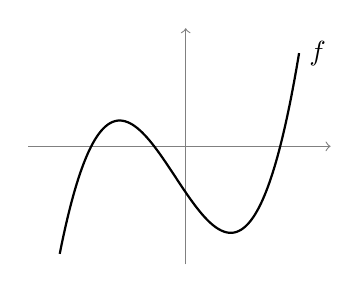
\begin{tikzpicture}[xscale=0.4,yscale=0.5]
\draw[->,thin,gray] (-5,0)--(4.6,0);
\draw[->,thin,gray] (0,-3)--(0,3);
\draw [thick,smooth,samples=100,variable=\x,domain=-4:3.6] plot(\x,{(\x+1)*(\x-3)*(\x+3)*0.13}) node[right] {$f$};
\end{tikzpicture}
\qquad\
\begin{tikzpicture}[xscale=0.4,yscale=0.5]
\draw[->,thin,gray] (-5,0)--(4.6,0);
\draw[->,thin,gray] (0,-3)--(0,3);
\draw [thick,smooth,samples=100,variable=\x,domain=-3:-1] plot(\x,{(\x+1)*(\x-3)*(\x+3)*0.13});
\draw [thick,smooth,samples=100,variable=\x,domain=3:3.6] plot(\x,{(\x+1)*(\x-3)*(\x+3)*0.13}) node[right] {$f^+$};
\draw [thick] (-4,0)--(-3,0);
\draw [thick] (-1,0)--(3,0);
\end{tikzpicture}
\qquad\
\begin{tikzpicture}[xscale=0.4,yscale=0.5]
\draw[->,thin,gray] (-5,0)--(4.6,0);
\draw[->,thin,gray] (0,-3)--(0,3);
\draw [thick,smooth,samples=100,variable=\x,domain=-4:-3] plot(\x,{-(\x+1)*(\x-3)*(\x+3)*0.13});
\draw [thick,smooth,samples=100,variable=\x,domain=-1:3] plot(\x,{-(\x+1)*(\x-3)*(\x+3)*0.13}) node[above=20pt] {$\ f^-$};
\draw [thick] (-3,0)--(-1,0);
\draw [thick] (3,0)--(3.7,0);
\end{tikzpicture}
\end{equation*}
Observe that $f=f^+-f^-$ and $|f|=f^++f^-$. Clearly, we have $f^+\leq|f|$ and $f^-\leq |f|$, and hence


\begin{equation*}
\int_{M}\!|f|\,\d \mu < \infty\quad \Leftrightarrow \quad \int_{M}\!f^+\,\d \mu < \infty\ \text{ and } \int_{M}\!f^-\,\d \mu < \infty.
\end{equation*}


\begin{definition}
Let $(M,\Sigma,\mu)$ be a measure space and let $f\cl M\to\overline{\R}$ be integrable. Then, the \emph{(Lebesgue) integral}\index{Lebesgue integral} of $f$ over $M$ with respect to $\mu$ is
\begin{equation*}
\int_{M}\!f\,\d \mu := \int_{M}\!f^+\,\d \mu -\int_{M}\!f^-\,\d \mu .
\end{equation*}
\end{definition}

It should be clear that the role of the integrability condition $\int_M |f|\, \d \mu<\infty$ is to prevent the integral of $f$ from being $\infty-\infty$, which is not defined.

In quantum mechanics, we usually deal with complex functions. The extension to the complex case of the integration theory presented thus far is straightforward.

\begin{definition}
Let $(M,\Sigma,\mu)$ be a measure space. A complex function $f\cl M\to\C$ is said to be \emph{integrable} if the real functions $\Re(f)$ and $\Im(f)$ are measurable and
\begin{equation*}
\int_{M}\!|f|\,\d \mu < \infty,
\end{equation*}
where $|f|$ denotes the complex modulus, i.e.\ $|f|^2=\Re(f)^2+\Im(f)^2$. We denote the set of all integrable complex functions by $\mathscr{L}^1_{\C}(M,\Sigma,\mu)$, or simply $\mathscr{L}^1(M)$ if there is no risk of confusion.
\end{definition}

\begin{definition}
Let $(M,\Sigma,\mu)$ be a measure space and let $f\cl M\to\C$ be integrable. We define
\begin{equation*}
\int_{M}\!f\,\d \mu := \int_{M}\!\Re(f)\,\d \mu +\mathrm{i}\int_{M}\!\Im(f)\,\d \mu .
\end{equation*}
\end{definition}

The following lemma gives the properties expected of sums and scalar
multiples of integrals. Note, however, that before we show that, say,
the integral of a sum is the sum of the integrals, it is necessary to
first show that the sum of two functions in $\mathscr{L}^1(M)$ is
again in $\mathscr{L}^1(M)$.

\begin{lemma}
\label{lem:l1vs}
Let $(M,\Sigma,\mu)$ be a measure space, let $f,g \in \mathscr{L}^1(M)$ and let $c \in \R$. Then
\begin{enumerate}[label=(\roman*)]
\item $|f| \in \mathscr{L}^1(M)$ and $ \displaystyle \biggl| \int_M \! f \, \d \mu \biggr| \leq \int_M \! | f| \, \d \mu $
\item $c f \in \mathscr{L}^1(M)$ and $ \displaystyle \int_M \! cf \, \d \mu = c \int_M \!  f \, \d \mu$
\item $f+g \in \mathscr{L}^1(M)$ and $ \displaystyle \int_M \! (f+g) \, \d \mu = \int_M \!  f \, \d \mu +  \int_M \!  g \, \d \mu$
\item $\mathscr{L}^1(M)$ is a vector space.
\end{enumerate}
\end{lemma}

\begin{proof}
\begin{enumerate}[label=(\roman*)]
\item As $\bigl| |f| \bigr|=|f|$, we have $|f| \in \mathscr{L}^1(M)$. Then, by the triangle inequality,
\begin{align*}
\left|  \int_M \! f \, \d \mu \right|
&= \left|  \int_M \! f^+ \, \d \mu -   \int_M \! f^- \, \d \mu \right|\\
& \leq \left|  \int_M \! f^+ \, \d \mu  \right| + \left| \int_M \! f^- \, \d \mu \right|\\
&=  \int_M \! f^+ \, \d \mu + \int_M \! f^- \, \d \mu \\
&=  \int_M \! (f^+ + f^-)\, \d \mu  \\
&= \int_M \!  |f| \, \d \mu.
\end{align*}
\item We have
\begin{equation*}
\int_M \!  |c f| \, \d \mu = \int_M \!  |c||f| \, \d \mu = |c|\int_M \!  | f| \, \d \mu< \infty
\end{equation*}
and hence, we have $c f \in \mathscr{L}^1(M)$.

\noindent Suppose $c \geq 0$. Then, $(c f)^+ = cf^+$ and $(c f)^- = c f^-$ and thus
\begin{align*}
  \int_M \!c f \, \d \mu
  &= \int_M \! (c f)^+ \, \d \mu -   \int_M \! (c f)^- \, \d \mu\\
  &= \int_M \! c f^+ \, \d \mu -   \int_M \! c f^- \, \d \mu\\
  &=  c\int_M \! f^+ \, \d \mu -c \int_M \! f^- \, \d \mu \\
  &=  c\int_M \! (f^+ -f^-)\, \d \mu  \\
  &= c\int_M \!  f \, \d \mu
\end{align*}
Now suppose $c = -1$. Then, $(- f)^+ = f^-$ and $(- f)^- = f^+$. Thus
\begin{align*}
  \int_M \! (-f) \, \d \mu
  &= \int_M \! (- f)^+ \, \d \mu -   \int_M \! (- f)^- \, \d \mu\\
  &= \int_M \! f^- \, \d \mu -   \int_M \!  f^+ \, \d \mu\\
  &= -\biggl( \int_M \! f^+ \, \d \mu - \int_M \! f^- \, \d \mu \biggr) \\
  &=  -\int_M \! (f^+ -f^-)\, \d \mu  \\
  &= -\int_M \!  f \, \d \mu.
\end{align*}
The case $c < 0$ follows by writing $c = (-1)(-c) $ and applying the above results.
\item By the triangle inequality, we have $|f+g| \leq | f| +| g|$ and thus
\begin{equation*}
\int_M \!  |f+g| \, \d \mu \leq \int_M \!  |f| \, \d \mu + \int_M \!  |g| \, \d \mu < \infty.
\end{equation*}
Hence, $f+g \in \mathscr{L}^1(M)$. Moreover, we have
\begin{equation*}
f+g = f^+ -f^- + g^+ -g^- = (f^++g^+)-(f^-+g^-),
\end{equation*}
where $f^++g^+$ and $f^-+g^-$ are non-negative and measurable. Note that, while $(f+g)^+\neq f^++g^+$ and $(f+g)^-\neq f^-+g^-$, one can show that $f^++g^+$ and $f^-+g^-$ give an equivalent splitting of $f+g$ to define its integral.
%with
% \begin{equation*}
% \int_M \! (f^-+g^-)\, \d \mu = \int_M \! f^- \, \d \mu + \int_M \! g^- \, \d \mu < \infty .
% \end{equation*}
Therefore
\begin{align*}
  \int_M \! (f+g) \, \d \mu
  &= \int_M \!  (f^++g^+) \, \d \mu - \int_M \! (f^-+g^-) \, \d \mu\\
  &= \int_M \!  f^+ \, \d \mu + \int_M \!  g^+ \, \d \mu - \int_M \! f^- \, \d \mu - \int_M \! g^- \, \d \mu   \\
  &=  \int_M \! (f^+ -f^-)\, \d \mu  + \int_M \! (g^+ -g^-)\, \d \mu\\
  &= \int_M \!  f \, \d \mu + \int_M \!  g \, \d \mu.
\end{align*}
\item The set of all functions from $M$ to $\overline{\R}$ is a vector space. By parts (ii) and (iii), we have that $\mathscr{L}^1(M)$ is a vector subspace of this vector space and hence, a vector space in its own right. \qedhere
\end{enumerate}
\end{proof}

Some properties of the integrals of non-negative, measurable functions easily carry over to general integrable functions.

\begin{lemma}
Let $(M,\Sigma,\mu)$ be a measure space and let $f,g \in \mathscr{L}^1(M)$. 
\begin{enumerate}[label=(\roman*)]
\item If $f=_{\mathrm{a.e.}}g$, then $\displaystyle \int_M\! f \, \d \mu = \int_M\! g \, \d \mu$
\item If $f\leq_{\mathrm{a.e.}}g$, then $\displaystyle \int_M\! f \, \d \mu \leq \int_M\! g \, \d \mu$.
\end{enumerate}
\end{lemma}

Just as the monotone convergence theorem was very important for integrals of non-negative, measurable functions, there is a similar theorem that is important for integrals of functions in $\mathscr{L}^1(X)$.

\begin{theorem}[Dominated convergence theorem]
Let $(M,\Sigma,\mu)$ be a measure space and let $\{f_n\}_{n\in\N}$ be a sequence of measurable functions which converges almost everywhere to a measurable function $f$. If there exists $g \in \mathscr{L}^1(M)$ such that $|f_n| \leq_{\mathrm{a.e.}} g$ for all $n \in \N$, then
\begin{enumerate}[label=(\roman*)]
\item $f \in \mathscr{L}^1(M)$ and $f_n \in \mathscr{L}^1(M)$ for all $n \in \N$
\item $\displaystyle \lim_{n \to \infty} \int_M \!  |f_n-f| \, \d \mu =0$
\item $\displaystyle \lim_{n \to \infty} \int_M \!  f_n \, \d \mu = \int_M \!  f \, \d \mu$.
\end{enumerate}
\end{theorem}

\begin{remark}
By ``$\{f_n\}_{n\in\N}$ converges almost everywhere to $f$'' we mean, of course, that there exists a null set $A\in\Sigma$ such that
\begin{equation*}
\forall \, m \in M\setminus A : \ \lim_{n\to\infty}f_n(m)=f(m).
\end{equation*}
\end{remark}


\section[\texorpdfstring{The function spaces $L^p(M,\Sigma,\mu)$}{The
function spaces Lp(M,Sigma,mu)}]{The function spaces $L^p(M,\Sigma,\mu)$}


While in quantum mechanics we need the theory of $L^p$ spaces only for $p=2$, it is worthwhile to develop the theory in more generality, by considering $L^p$ for all $1\leq p\leq \infty$.

\begin{definition}
Let $(M,\Sigma,\mu)$ be a measure space and let $p\in [1,\infty)$. We define
\begin{equation*}
\mathscr{L}^p_{\R}(M,\Sigma,\mu) := \biggl\{f\cl M \to \overline{\R}\ \Big| \ f \text{ is measurable and } \int_M\!|f|^p\,\d \mu < \infty\biggr\}
\end{equation*}
and, similarly,
\begin{equation*}
\mathscr{L}^p_{\C}(M,\Sigma,\mu)
:=
\biggl\{
f\cl M \to \C\
\Big|
\parbox{60mm}{\centering
\(\Re(f)\) and \(\Im(f)\) are measurable \\
and \(\int_M\!|f|^p\,\d \mu < \infty\)
}
\biggr\}.
\end{equation*}
Whenever there is no risk of confusion, we lighten the notation to just $\mathscr{L}^p$.
\end{definition}


\begin{definition}
Let $(M,\Sigma,\mu)$ be a measure space and let $f\cl M \to \overline{\R}$. The \emph{essential supremum}\index{essential supremum} of $f$ is defined as
\begin{equation*}
\esup%_M
f := \inf\{c\in\overline{\R}\mid f \leq_{\mathrm{a.e.}}c\}.
\end{equation*}
Then, $f$ is said to be \emph{almost everywhere bounded (from above)} if $\esup f < \infty$. 
\end{definition}

Alternatively, $f\cl M \to \overline{\R}$ is almost everywhere bounded if there exists a null set $A\in \Sigma$ such that $f$ restricted to $M\setminus A$ is bounded.

\begin{definition}
Let $(M,\Sigma,\mu)$ be a measure space. We define
\begin{equation*}
\mathscr{L}^{\infty}_{\R}(M,\Sigma,\mu) := \biggl\{f\cl M \to \overline{\R}\ \Big| \ f \text{ is measurable and } \esup |f| < \infty\biggr\}
\end{equation*}
and, similarly,
\begin{equation*}
\mathscr{L}^{\infty}_{\C}(M,\Sigma,\mu)
:= \biggl\{
f\cl M \to \C
\ \Big| \
\parbox{60mm}{\centering
\(\Re(f)\) and \(\Im(f)\) are measurable \\
and \(\esup |f| < \infty\)
}
\biggr\}.
\end{equation*}
Whenever there is no risk of confusion, we lighten the notation to just $\mathscr{L}^p$, for $p\in[1,\infty]$.
\end{definition}

All the $\mathscr{L}^p$ spaces become vector spaces once equipped with pointwise addition and multiplication. Let us show this is detail for $\mathscr{L}_{\C}^2$.

\begin{proposition}
Let $(M,\Sigma,\mu)$ be a measure space. Then, $\mathscr{L}_{\C}^2$ is a complex vector space.
\end{proposition}

\begin{proof}
The set of all functions $M\to\C$, often denoted $M^{\C}$, is a vector space under pointwise addition and multiplication. Hence, it suffices to show that $\mathscr{L}_{\C}^2$ is a subspace of $M^{\C}$.
\begin{enumerate}[label=(\roman*)]
\item Let $f \in \mathscr{L}_{\C}^2$ and $z\in \C$. As $|z|\in \R$, we have:
\begin{equation*}
\int_M \!  |z f|^2 \, \d \mu = |z|^2 \int_M \!  |f|^2 \, \d \mu < \infty
\end{equation*}
and hence, $z f \in \mathscr{L}_{\C}^2$.
\item Let $f,g \in \mathscr{L}_{\C}^2$. Note that
\begin{align*}
|f+g|^2 
&= (f+g)\overline{(f+g)}\\
&= (f+g)(\overline{f}+\overline{g})\\
&= f\overline{f}+f\overline{g}+g\overline{f}+g\overline{g} \\
&= |f|^2 +f\overline{g}+g\overline{f}+ |g|^2.
\end{align*}
Moreover, as
\begin{equation*}
0 \leq |f-g|^2 = |f|^2 -f\overline{g}-g\overline{f}+ |g|^2 ,
\end{equation*}
we have $f\overline{g}+g\overline{f} \leq |f|^2+ |g|^2$, and thus
\begin{equation*}
|f+g|^2 \leq 2 |f|^2+ 2|g|^2.
\end{equation*}
Therefore
\begin{equation*}
\int_M \!  |f+g|^2 \, \d \mu \leq 2\int_M \!  |f|^2 \, \d \mu + 2\int_M \!  |g|^2 \, \d \mu  < \infty ,
\end{equation*}
and hence $f+g \in \mathscr{L}_{\C}^2$.\qedhere
\end{enumerate}
\end{proof}

Ideally, we would like to turn all these $\mathscr{L}^p$ space into Banach spaces. Let us begin by equipping them with a weaker piece of extra structure.

\begin{proposition}
Let $(M,\Sigma,\mu)$ be a measure space and let $p\in[0,\infty]$. Then, the maps $\|\cdot\|_p\cl \mathscr{L}^p\to\R$ defined by
\begin{equation*}
\|f\|_p:=
\begin{cases}
\biggl(\displaystyle\int_M\! |f|^p\,\d \mu\biggr)^{\negmedspace\frac{1}{p}} & \text{ for } 1\leq p<\infty\\
\esup |f| & \text{ for }p=\infty
\end{cases}
\end{equation*}
are semi-norms on $\mathscr{L}^p$. That is, for all $z\in \C$ and $f,g\in\mathscr{L}^p$,
\begin{enumerate}[label=(\roman*)]
\item $\|f\|_p\geq 0$
\item $\|z f\|_p = |z|\|f\|_p$
\item $\|f+g\|_p\leq\|f\|_p+\|g\|_p$.
\end{enumerate}
\end{proposition}
In other words, the notion of semi-norm is a generalisation of that of norm obtained by relaxing the definiteness condition. If the measure space $(M,\Sigma,\mu)$ is such that the empty set is the only null set, then $\|\cdot\|_p$ is automatically definite and hence, a norm.

\begin{example}
Consider $(\N,\mathscr{P}(\N),\mu)$, where $\mu$ is the counting measure. Then, as $\mu(A)$ is the cardinality of $A$, the only null set is the empty set. Thus, recalling that functions on $\N$ are just sequences, the maps
\begin{equation*}
\|\{a_n\}_{n\in\N}\|_p = 
\begin{cases}
\biggl(\displaystyle\sum_{\,n=0}^{\infty} |a_n|^p\biggr)^{\negmedspace\frac{1}{p}} & \text{ for } 1\leq p<\infty\\
\sup \{|a_n| \mid n\in \N\} & \text{ for }p=\infty
\end{cases}
\end{equation*}
are norms on $\mathscr{L}^p(\N)$. In particular, note that we have $\mathscr{L}^2(\N)=\ell^2(\N)$.
\end{example}

However, in general measure spaces, we only have
\begin{equation*}
\|f\|_p = 0 \quad \Leftrightarrow \quad f =_{\mathrm{a.e.}} 0,
\end{equation*}
as we have shown in \Cref{thm:aezero} for $\mathscr{L}^1$, and it is often very easy to produce an $f\neq 0$ such that $\|f\|_p=0$. The solution to this problem is to construct new spaces from the $\mathscr{L}^p$ in which functions that are almost everywhere equal are, in fact, the same function. In other words, we need to consider the quotient space of $\mathscr{L}^p$ by the equivalence relation ``being almost everywhere equal''.

\begin{definition}
Let $M$ be a set. An \emph{equivalence relation} on $M$ is a set $\sim\ \subseteq M\times M$ such that, writing $a\sim b$ for $(a,b)\in\ \sim$, we have
\begin{enumerate}[label=(\roman*)]
\item $a\sim a$ \hfill (reflexivity)
\item $a\sim b \ \Leftrightarrow\ b\sim a$ \hfill (symmetry)
\item $(a \sim b \text{ and } b\sim c) \ \Rightarrow \ a\sim c$ \hfill (transitivity)
\end{enumerate}
for all $a,b,c\in M$. If $\sim$ is an equivalence relation on $M$, we define the \emph{equivalence class} of $m\in M$ by $[m]:=\{a\in M \mid m\sim a\}$ and the \emph{quotient set} of $M$ by $\sim$ by
\begin{equation*}
M/{\sim} := \{[m]\mid m\in M\}.
\end{equation*}
\end{definition}
It is easy to show that $M/{\sim}$ is a \emph{partition} of $M$, i.e.\
\begin{equation*}
M = \bigcup_{m\in M}[m] \qquad \text{and}\qquad [a]\cap [b]=\varnothing \text{ whenever } a\neq b.
\end{equation*}
In fact, the notions of equivalence relation on $M$ and partition of $M$ are one and the same.

\begin{lemma}
Let $(M,\Sigma,\mu)$ be a measure space and let $\sim$ be defined by
\begin{equation*}
f\sim g \quad :\Leftrightarrow \quad f=_{\mathrm{a.e.}}g.
\end{equation*}
Then, $\sim$ is an equivalence relation on $\mathscr{L}^p$.
\end{lemma}

\begin{proof}
Let $f,g,h\in\mathscr{L}^p$. Clearly, $f\sim f$ and $f\sim g \Leftrightarrow g \sim f$. Now suppose that $f\sim g$ and $g\sim h$. Then, there exist null sets $A,B\in\Sigma$ such that $f=g$ on $M\setminus A$ and $g=h$ on $M\setminus B$. Recall that $\sigma$-algebras are closed under intersections and hence, $A\cap B\in\Sigma$. Obviously, we have $f=h$ on $M\setminus (A\cap B)$ and, since
\begin{equation*}
\mu(A\cap B) \leq \mu (A\cup B) \leq \mu(A)+\mu(B) = 0,
\end{equation*}
the set $A\cap B$ is null. Thus, $f\sim h$.
\end{proof}


\begin{definition}
Let $(M,\Sigma,\mu)$ be a measure space and let $f\sim g \Leftrightarrow f=_{\mathrm{a.e.}}g $. We define
\begin{equation*}
L^p := \mathscr{L}^p/{\sim} = \{[f]\mid f\in \mathscr{L}^p\}.
\end{equation*}
\end{definition}

\begin{lemma}
Let $(M,\Sigma,\mu)$ be a measure space. Then, the maps
\begin{enumerate}[label=(\roman*)]
\item $+\cl L^p\times L^p \to L^p$ defined by $[f]+[g]:=[f+g]$
\item $\cdot\cl \C\times L^p \to L^p$ defined by $z[f]:=[zf]$
\item $\|\cdot\|_p\cl L^p \to \R$ defined by $\|[f]\|_p:=\|f\|_p$
\end{enumerate}
are well-defined. Moreover, $\|\cdot\|_p\cl L^p \to \R$ is a norm on $L^p$.
\end{lemma}

\begin{lemma}[H\"older's inequality]
Let $(M,\Sigma,\mu)$ be a measure space and let $p,q\in[1,\infty]$ be such that $\tfrac{1}{p}+\tfrac{1}{q}=1$ (where $\tfrac{1}{\infty}:=0$). Then, for all measurable functions $f,g\cl M\to \C$, we have
\begin{equation*}
\biggl|\int_M\!fg \, \d \mu \biggr| \leq \biggl(\int_M\!|f|^p \, \d \mu\biggr)^{\negmedspace \frac{1}{p}}\biggl(\int_M\!|g|^q \, \d \mu\biggr)^{\negmedspace \frac{1}{q}}.
\end{equation*}
\end{lemma}

Hence, if $[f]\in L^p$ and $[g]\in L^q$, with  $\tfrac{1}{p}+\tfrac{1}{q}=1$ , then $[fg]\in L^1$ and
\begin{equation*}
\|[fg]\|_1\leq\|[f]\|^p\|[g]\|^q.
\end{equation*}

\begin{theorem}
The spaces $L^p$ are Banach spaces for all $p\in[0,\infty]$.
\end{theorem}

We have already remarked that the case $p=2$ is special in that $L^2$ is the only $L^p$ space which can be made into a Hilbert space.

\begin{proposition}
Let $(M,\Sigma,\mu)$ be a measure space and define
\begin{IEEEeqnarray*}{rrCl}
\langle\cdot|\cdot\rangle_{L^2} \cl & L^2\times L^2 & \to & \C\\
& ([f],[g]) & \mapsto & \displaystyle \int_M\!\overline{f}g\, \d \mu.
\end{IEEEeqnarray*}
Then, $\langle\cdot|\cdot\rangle_{L^2} $ is well-defined and it is a sesqui-linear inner product on $L^2$.
\end{proposition}

\begin{proof}
First note that if $[f]\in L^2$, then $[\overline{f}]\in L^2$ and hence, by H\"older inequality, $[\overline{f}g]\in L^1$. This ensures that $\bigl\langle [f]\big|[g]\bigr\rangle_{L^2}\in \C$ for all $[f],[g]\in L^2$.

To show well-definedeness, let $f'=_{\mathrm{a.e.}}f$ and $g'=_{\mathrm{a.e.}}g$. Then, $\overline{f'}g'=_{\mathrm{a.e.}}\overline{f}g$ and thus
\begin{equation*}
\bigl\langle [f']\big|[g']\bigr\rangle_{L^2} :=  \int_M\!\overline{f'}g'\, \d \mu =  \int_M\!\overline{f}g\, \d \mu =: \bigl\langle [f]\big|[g]\bigr\rangle_{L^2} .
\end{equation*}

Now, let $[f],[g],[h]\in L^2$ and $z\in \C$. Then
\begin{enumerate}[label=(\roman*)]
\item $\displaystyle\overline{\bigl\langle [f]\big|[g]\bigr\rangle}_{L^2} = \overline{\int_M\!\overline{f}g\, \d \mu} = \int_M\!f\overline{g}\, \d \mu = \bigl\langle [g]\big|[f]\bigr\rangle_{L^2}$
\item We have
\begin{IEEEeqnarray*}{rCl}
\bigl\langle [f]\big|z[g]+[h]\bigr\rangle_{L^2} & = & \int_M\!\overline{f}(zg+h)\, \d \mu \\
& = & z\int_M\!\overline{f}g\, \d \mu+\int_M\!\overline{f}h\, \d \mu \\
& = & z\bigl\langle [f]\big|[g]\bigr\rangle_{L^2}+\bigl\langle [f]\big|[h]\bigr\rangle_{L^2}
\end{IEEEeqnarray*}
\item We have $\displaystyle\bigl\langle [f]\big|[f]\bigr\rangle_{L^2} = \int_M\!\overline{f}f\, \d \mu = \int_M\!|f|^2\, \d \mu \geq 0 $ and
\begin{equation*}
\bigl\langle [f]\big|[f]\bigr\rangle_{L^2} = 0 \quad \Leftrightarrow \quad \int_M\!|f|^2\, \d \mu = 0  \quad \Leftrightarrow \quad \|[f]\|_2 = 0.
\end{equation*}
Thus, $[f]=0:=[0]$. \qedhere
\end{enumerate}
\end{proof}

The last part of the proof also shows that $\langle\cdot | \cdot \rangle_{L^2}$ induces the norm $\|\cdot\|_2$, with respect to which $L^2$ is a Banach space. Hence, $(L^2,\langle\cdot | \cdot \rangle_{L^2})$ is a Hilbert space.

\begin{remark}
The inner product $\langle\cdot | \cdot \rangle_{L^2}$ on $L^2_{\C}(\N,\mathscr{P}(\N),\mu)$ coincides with the inner product $\langle\cdot | \cdot \rangle_{\ell^2}$ on $\ell^2(\N)$ defined in the section on separable Hilbert spaces.
\end{remark}























